\chapter{Kết quả thực nghiệm}
\label{chap:results}

\section{Thiết lập thực nghiệm}
\label{sec:experimental_setup}

Toàn bộ thực nghiệm sử dụng dữ liệu IMU 6 trục (gia tốc kế + con quay hồi chuyển) được thu thập từ một đối tượng trên thiết bị Seeed XIAO nRF52840 Sense (IMU LSM6DS3 tích hợp) ở tần số lấy mẫu 100~Hz. Dữ liệu gồm các bản ghi 30--60 giây cho mỗi hoạt động. Hai cấu hình bài toán được đánh giá:
\begin{itemize}
    \item \textbf{Bài toán 3 lớp}: running, still, walking --- ba hoạt động có đặc điểm sinh cơ học khác biệt rõ rệt
    \item \textbf{Bài toán 5 lớp}: running, still, walking, walking\_downstairs, walking\_upstairs --- bổ sung hai hoạt động có dấu hiệu chuyển động tương tự nhau (leo và xuống cầu thang so với đi bộ thường)
\end{itemize}

Các tham số chung: kích thước cửa sổ $W = 150$ mẫu (1,5 giây), bước trượt $S = 75$ mẫu (50\% chồng lấp), đệm cửa sổ bằng lặp giá trị biên (edge-value replication). Tăng cường dữ liệu (augmentation) với hệ số 2 sử dụng ba phương pháp (jitter, rotation, scaling). Chia dữ liệu: 70\% huấn luyện, 15\% xác thực, 15\% kiểm tra, sử dụng phân chia phân tầng (stratified split). Loại đặc trưng sử dụng: \texttt{orientation\_invariant} (63 đặc trưng: thống kê thời gian trên acc\_mag, gyro\_mag, acc\_jerk\_mag cộng với đặc trưng phổ DFT trên acc\_mag và gyro\_mag); riêng CNN sử dụng đầu vào thô 6 trục ($150 \times 6$).

Năm thuật toán được đánh giá: Neural Network (sklearn MLP), Random Forest, SVM (RBF kernel), PyTorch MLP và PyTorch 1D-CNN. Tất cả các mô hình sử dụng cân bằng trọng số lớp (\texttt{class\_weight='balanced'}) khi áp dụng được.

\section{Kết quả huấn luyện}
\label{sec:training_results}

\subsection{Bài toán 3 lớp (running / still / walking)}
\label{sec:three_class}

Bảng~\ref{tab:3class_accuracy} tóm tắt kết quả huấn luyện cho bài toán 3 lớp. Ba hoạt động này có đặc trưng sinh cơ học phân biệt rõ rệt: running có biên độ gia tốc cao và tần số bước nhanh; still gần như bất động với magnitude gia tốc ổn định quanh $g$; walking có biên độ trung gian với tần số bước đặc trưng.

\begin{table}[H]
    \centering
    \caption{Kết quả huấn luyện --- bài toán 3 lớp (63 đặc trưng orientation-invariant, tập kiểm tra 156 mẫu)}
    \label{tab:3class_accuracy}
    \resizebox{\textwidth}{!}{
    \begin{tabular}{@{}lccccc@{}}
        \toprule
        Thuật toán & Kiến trúc / Cấu hình & \makecell{Thời gian\\huấn luyện (s)} & \makecell{Độ chính xác\\huấn luyện (\%)} & \makecell{Độ chính xác\\xác thực (\%)} & \makecell{Độ chính xác\\kiểm tra (\%)} \\
        \midrule
        Neural Network & 63--100--50--3 & 0,22 & 99,17 & 100,00 & 100,00 \\
        Random Forest & 50 cây, sâu tối đa 10 & 0,12 & 100,00 & --- & 100,00 \\
        SVM (RBF) & $C\!=\!1$, $\gamma\!=\!\text{scale}$ & 0,09 & 100,00 & --- & 100,00 \\
        PyTorch MLP & 63--ẩn--3 & 2,54 & 99,86 & 100,00 & 100,00 \\
        PyTorch 1D-CNN & $150 \times 6$ thô & 10,29 & 100,00 & 100,00 & 100,00 \\
        \bottomrule
    \end{tabular}}
\end{table}

Tất cả năm thuật toán đạt 100\% độ chính xác trên tập kiểm tra cho bài toán 3 lớp, với F1-score = 1,0 trên mọi lớp. Kết quả này xác nhận rằng ba hoạt động cơ bản (chạy, đứng yên, đi bộ) có thể được phân biệt hoàn toàn bằng 63 đặc trưng bất biến hướng. Đáng chú ý, thời gian huấn luyện của các mô hình cổ điển (0,09--0,22 giây) nhanh hơn đáng kể so với PyTorch (2,54--10,29 giây), cho thấy lợi thế của ML cổ điển khi bài toán không quá phức tạp.

\subsection{Bài toán 5 lớp --- Đánh giá chính}
\label{sec:five_class}

Bài toán 5 lớp bổ sung walking\_downstairs và walking\_upstairs --- hai hoạt động có cấu trúc bước tương tự đi bộ thường nhưng khác nhau về thành phần xoay và biên độ gia tốc thẳng đứng. Đây là bài toán thách thức hơn đáng kể, thể hiện đúng hơn các yêu cầu thực tế. Bảng~\ref{tab:5class_accuracy} trình bày kết quả.

\begin{table}[H]
    \centering
    \caption{Kết quả huấn luyện --- bài toán 5 lớp (63 đặc trưng orientation-invariant, tập kiểm tra 229 mẫu)}
    \label{tab:5class_accuracy}
    \resizebox{\textwidth}{!}{
    \begin{tabular}{@{}lccccc@{}}
        \toprule
        Thuật toán & Kiến trúc / Cấu hình & \makecell{Thời gian\\huấn luyện (s)} & \makecell{Độ chính xác\\huấn luyện (\%)} & \makecell{Độ chính xác\\xác thực (\%)} & \makecell{Độ chính xác\\kiểm tra (\%)} \\
        \midrule
        Neural Network & 63--100--50--5 & 0,42 & 99,72 & 98,25 & 98,69 \\
        Random Forest & 50 cây, sâu tối đa 10 & 0,15 & 99,81 & --- & 98,25 \\
        SVM (RBF) & $C\!=\!1$, $\gamma\!=\!\text{scale}$ & 0,15 & 97,55 & --- & 97,38 \\
        PyTorch MLP & 63--ẩn--5 & 1,94 & 99,81 & 98,69 & 99,13 \\
        PyTorch 1D-CNN & $150 \times 6$ thô & 10,09 & 99,25 & 99,56 & 99,13 \\
        \bottomrule
    \end{tabular}}
\end{table}

Khi mở rộng từ 3 lên 5 lớp, độ chính xác kiểm tra giảm từ 100\% xuống 97,38--99,13\%, phản ánh độ khó phân biệt giữa các hoạt động liên quan (walking vs walking\_upstairs/downstairs). Các quan sát chính:
\begin{itemize}
    \item \textbf{PyTorch MLP và 1D-CNN} đạt độ chính xác cao nhất (99,13\%), cho thấy lợi thế của các kiến trúc học sâu khi bài toán phức tạp hơn.
    \item \textbf{Neural Network (sklearn)} đạt 98,69\% với thời gian huấn luyện chỉ 0,42 giây --- cân bằng tốt giữa hiệu suất và tốc độ phát triển.
    \item \textbf{SVM} có độ chính xác thấp nhất (97,38\%), với độ chính xác huấn luyện cũng chỉ 97,55\% --- gợi ý rằng kernel RBF với cấu hình mặc định chưa nắm bắt đủ cấu trúc phi tuyến của bài toán 5 lớp; tối ưu hóa siêu tham số có thể cải thiện đáng kể.
    \item \textbf{1D-CNN} hoạt động trên dữ liệu thô mà không cần trích xuất đặc trưng thủ công, đạt hiệu suất ngang PyTorch MLP nhưng tốn thời gian huấn luyện nhiều hơn (10,09 giây).
\end{itemize}

\subsection{Hiệu suất theo từng lớp}
\label{sec:per_class_results}

Bảng~\ref{tab:perclass_5class} trình bày chi tiết precision, recall và F1-score cho từng lớp hoạt động trên bài toán 5 lớp. Ba thuật toán đại diện cho ba nhóm tiếp cận (ML cổ điển: RF; neural truyền thống: NN; học sâu: PyTorch MLP) được so sánh.

\begin{table}[H]
    \centering
    \caption{Hiệu suất theo từng lớp --- bài toán 5 lớp, tập kiểm tra (229 mẫu)}
    \label{tab:perclass_5class}
    \resizebox{\textwidth}{!}{
    \begin{tabular}{@{}l ccc ccc ccc@{}}
        \toprule
        & \multicolumn{3}{c}{Neural Network (98,69\%)} & \multicolumn{3}{c}{Random Forest (98,25\%)} & \multicolumn{3}{c}{PyTorch MLP (99,13\%)} \\
        \cmidrule(lr){2-4} \cmidrule(lr){5-7} \cmidrule(lr){8-10}
        Hoạt động & P & R & F1 & P & R & F1 & P & R & F1 \\
        \midrule
        Running (56) & 1,000 & 1,000 & 1,000 & 1,000 & 1,000 & 1,000 & 1,000 & 1,000 & 1,000 \\
        Still (51) & 1,000 & 1,000 & 1,000 & 1,000 & 1,000 & 1,000 & 1,000 & 1,000 & 1,000 \\
        Walking (49) & 1,000 & 0,980 & 0,990 & 0,979 & 0,959 & 0,969 & 1,000 & 0,980 & 0,990 \\
        W.\ Downstairs (38) & 0,949 & 0,974 & 0,961 & 0,925 & 0,974 & 0,949 & 0,950 & 1,000 & 0,974 \\
        W.\ Upstairs (35) & 0,971 & 0,971 & 0,971 & 1,000 & 0,971 & 0,986 & 1,000 & 0,971 & 0,986 \\
        \midrule
        \textbf{Macro Avg} & \textbf{0,984} & \textbf{0,985} & \textbf{0,984} & \textbf{0,981} & \textbf{0,981} & \textbf{0,981} & \textbf{0,990} & \textbf{0,990} & \textbf{0,990} \\
        \bottomrule
    \end{tabular}}
    \begin{minipage}{\linewidth}
    \vspace{4pt}
    \footnotesize
    P = Precision, R = Recall. Số trong ngoặc = số mẫu kiểm tra (support). W.\ = Walking.
    \end{minipage}
\end{table}

Phân tích theo từng lớp cho thấy các mẫu phân loại sai tập trung ở nhóm hoạt động đi bộ:
\begin{itemize}
    \item \textbf{Running và Still} đạt F1 = 1,000 trên tất cả các thuật toán --- dấu hiệu sinh cơ học đặc trưng (biên độ gia tốc cao cho running, magnitude ổn định quanh $g$ cho still) tạo ranh giới phân loại rõ ràng.
    \item \textbf{Walking Downstairs} có precision thấp nhất (0,925--0,950), nghĩa là một số mẫu từ lớp khác (chủ yếu walking) bị phân loại nhầm thành walking\_downstairs --- phù hợp với đặc điểm rằng đi bộ thường và xuống cầu thang chia sẻ biên độ gia tốc tương tự.
    \item \textbf{Walking Upstairs} đạt recall 0,971 nhất quán trên mọi thuật toán --- một vài mẫu bị nhầm lẫn với walking thường, nhưng precision cao (0,971--1,000) cho thấy khi mô hình dự đoán walking\_upstairs thì hầu như luôn đúng.
\end{itemize}

Kết quả tổng thể xác nhận rằng loại đặc trưng \texttt{orientation\_invariant} có khả năng phân biệt tốt giữa 5 hoạt động, với sai sót chủ yếu ở ranh giới giữa các dạng đi bộ --- nơi sự khác biệt chủ yếu nằm ở thành phần xoay (vận tốc góc gập cổ chân) mà đặc trưng tổng hợp magnitude bắt giữ nhưng không hoàn toàn tách biệt. Hình~\ref{fig:confusion_5class_mlp} minh họa ma trận nhầm lẫn trực quan cho mô hình PyTorch MLP --- thuật toán đạt F1 cao nhất (0,990) trên đặc trưng thủ công.

\begin{figure}[H]
    \centering
    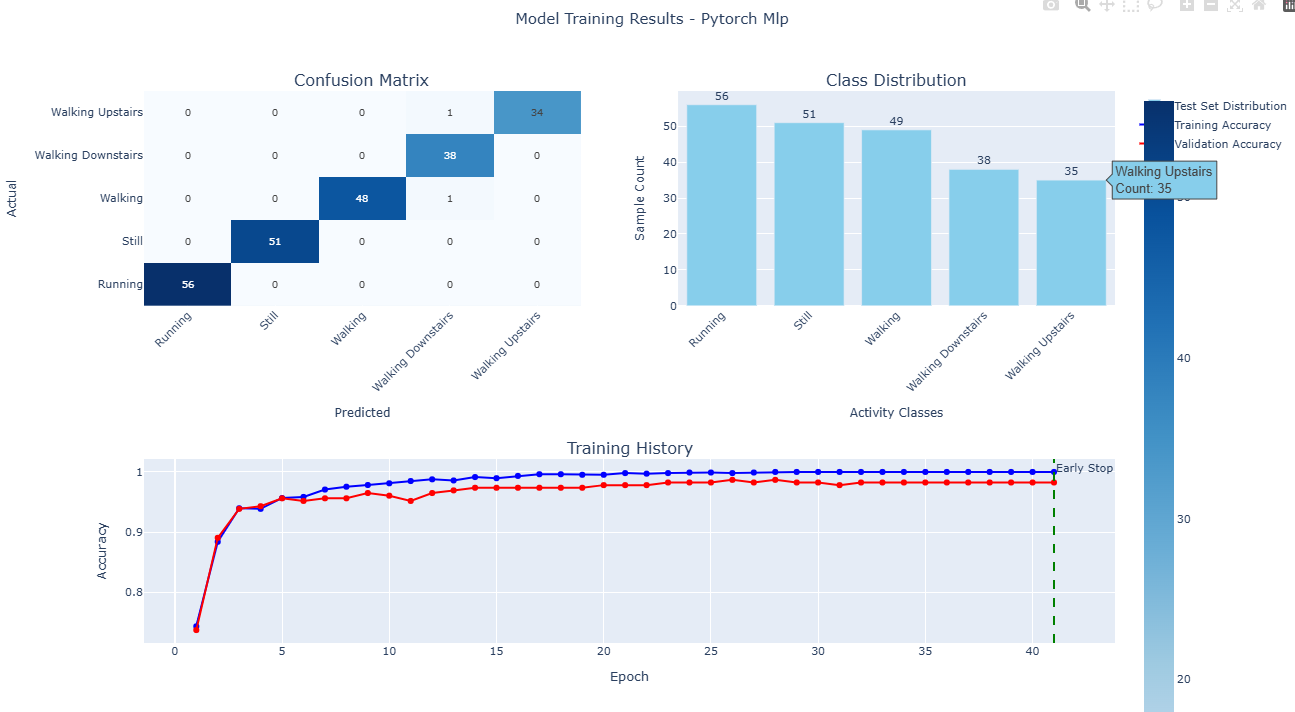
\includegraphics[width=0.7\textwidth]{figures/ui_mlp_training_c5_confusion.png}
    \caption{Ma trận nhầm lẫn --- PyTorch MLP, bài toán 5 lớp (tập kiểm tra 229 mẫu). Các lỗi phân loại tập trung ở nhóm hoạt động đi bộ: 1 mẫu walking bị nhầm thành walking\_downstairs (hàng walking, cột W.Down).}
    \label{fig:confusion_5class_mlp}
\end{figure}

\section{So sánh hiệu suất giữa các thuật toán}
\label{sec:algorithm_comparison}

Bảng~\ref{tab:algorithm_comparison} tổng hợp so sánh trên nhiều tiêu chí cho bài toán 5 lớp.

\begin{table}[H]
    \centering
    \caption{So sánh tổng hợp các thuật toán --- bài toán 5 lớp}
    \label{tab:algorithm_comparison}
    \resizebox{\textwidth}{!}{
    \begin{tabular}{@{}lccccl@{}}
        \toprule
        Thuật toán & \makecell{Độ chính xác\\kiểm tra (\%)} & \makecell{Macro\\F1} & \makecell{Thời gian\\huấn luyện (s)} & \makecell{Đầu vào\\(số chiều)} & Nhận xét \\
        \midrule
        PyTorch MLP & 99,13 & 0,990 & 1,94 & 63 & Tốt nhất trên đặc trưng thủ công \\
        PyTorch 1D-CNN & 99,13 & 0,992 & 10,09 & $150\!\times\!6$ & End-to-end, không cần FE \\
        Neural Network & 98,69 & 0,984 & 0,42 & 63 & Nhanh, đủ tốt cho prototyping \\
        Random Forest & 98,25 & 0,981 & 0,15 & 63 & Nhanh nhất, không cần chuẩn hóa \\
        SVM (RBF) & 97,38 & 0,972 & 0,15 & 63 & Cần tối ưu hóa siêu tham số \\
        \bottomrule
    \end{tabular}}
\end{table}

Biên độ chênh lệch giữa thuật toán tốt nhất (PyTorch MLP/CNN: 99,13\%) và thấp nhất (SVM: 97,38\%) chỉ 1,75 điểm phần trăm --- cho thấy chất lượng pipeline trích xuất đặc trưng quan trọng hơn lựa chọn thuật toán khi đặc trưng đã được thiết kế tốt. Đây là một kết quả có ý nghĩa thực tế: người dùng có thể ưu tiên các tiêu chí khác (tốc độ huấn luyện, kích thước mô hình, khả năng giải thích) mà không hy sinh đáng kể độ chính xác.

Ảnh hưởng của số lượng lớp đến hiệu suất được tóm tắt trong Bảng~\ref{tab:class_scaling}.

\begin{table}[H]
    \centering
    \caption{Ảnh hưởng của số lượng lớp đến độ chính xác kiểm tra}
    \label{tab:class_scaling}
    \begin{tabular}{@{}lccc@{}}
        \toprule
        Thuật toán & 3 lớp (\%) & 5 lớp (\%) & Giảm (điểm \%) \\
        \midrule
        Neural Network & 100,00 & 98,69 & $-1{,}31$ \\
        Random Forest & 100,00 & 98,25 & $-1{,}75$ \\
        SVM (RBF) & 100,00 & 97,38 & $-2{,}62$ \\
        PyTorch MLP & 100,00 & 99,13 & $-0{,}87$ \\
        PyTorch 1D-CNN & 100,00 & 99,13 & $-0{,}87$ \\
        \bottomrule
    \end{tabular}
\end{table}

Các mô hình PyTorch giảm ít nhất ($-0{,}87$ điểm), trong khi SVM giảm nhiều nhất ($-2{,}62$ điểm). Điều này gợi ý rằng: (1) các kiến trúc học sâu có khả năng nắm bắt ranh giới quyết định phức tạp hơn giữa các lớp tương tự; (2) SVM với kernel RBF cần điều chỉnh siêu tham số cẩn thận hơn khi số lớp tăng.

\section{Khả năng triển khai đa thiết bị}
\label{sec:multi_device}

Đóng góp cốt lõi của framework không chỉ nằm ở độ chính xác mô hình, mà ở khả năng sử dụng cùng một mô hình đã huấn luyện để sinh mã triển khai cho nhiều họ thiết bị khác nhau mà không cần huấn luyện lại. Bảng~\ref{tab:deployment_matrix} tóm tắt ma trận đích triển khai được hỗ trợ.

\begin{table}[H]
    \centering
    \caption{Ma trận đích triển khai --- phạm vi hỗ trợ của hệ thống tạo mã}
    \label{tab:deployment_matrix}
    \small
    \begin{tabular}{@{}p{2.8cm}p{3.5cm}p{2.0cm}p{4.0cm}@{}}
        \toprule
        Nhóm đích & Nền tảng cụ thể & Ngôn ngữ & Phạm vi xác thực \\
        \midrule
        Arduino-compatible & Seeed XIAO, ESP32, M5Stack, Teensy & C++ & Benchmark chi tiết trên XIAO \\
        ARM Cortex-M & Generic ARM Cortex-M & C & Xác minh biên dịch + cấu trúc \\
        SDK/RTOS & ESP-IDF, Zephyr, Generic C/C++ & C/C++ & Xác minh tạo mã \\
        MicroPython & Vi điều khiển hỗ trợ MPy & Python & Xác minh tương đồng công thức \\
        Runtime thay thế & TFLite Micro, ONNX Runtime & C++ + nhị phân & Chỉ NN/CNN \\
        \bottomrule
    \end{tabular}
\end{table}

Kiến trúc tạo mã phân tách ba lớp --- mô hình ML, nền tảng đích, backend triển khai --- cho phép tổ hợp linh hoạt: một Random Forest đã huấn luyện có thể được xuất đồng thời sang C++ cho Arduino, C cho ARM Cortex-M, và Python cho MicroPython, từ cùng một tệp \texttt{.joblib}. Bốn chế độ tối ưu hóa (\texttt{accuracy}, \texttt{balanced}, \texttt{speed}, \texttt{power}) điều chỉnh độ chính xác số học (số chữ số thập phân cho trọng số và tham số chuẩn hóa) và chiến lược bộ đệm theo ràng buộc tài nguyên của nền tảng đích.

\textbf{Giới hạn backend runtime thay thế}: TFLite Micro và ONNX Runtime chỉ hỗ trợ trực tiếp Neural Network và CNN. Random Forest và SVM không thể chuyển đổi qua đường dẫn ONNX $\to$ TFLite vì các toán tử ONNX-ML (\texttt{TreeEnsembleClassifier}, \texttt{SVMClassifier}) không được \texttt{onnx2tf} hỗ trợ. Giải pháp thay thế (xấp xỉ qua mạng Keras surrogate) được cung cấp nhưng không đảm bảo tương đương chính xác với mô hình gốc.

\section{Đánh giá triển khai trên thiết bị}
\label{sec:device_benchmark}

Để đánh giá hiệu suất triển khai thực tế, mã C++ được sinh ra cho từng mô hình được biên dịch và nạp lên thiết bị Seeed XIAO nRF52840 Sense (ARM Cortex-M4F @ 64~MHz, 1~MB flash, 256~KB RAM). Kiểm tra được thực hiện bằng cách thực hiện từng hoạt động và quan sát kết quả phân loại thời gian thực qua giao diện Serial. Ngưỡng tin cậy $\tau = 0{,}6$ được sử dụng.

\subsection{Tổng hợp kết quả triển khai}
\label{sec:deployment_results}

Bảng~\ref{tab:deployment_status} tóm tắt kết quả triển khai cho cả hai cấu hình bài toán.

\begin{table}[H]
    \centering
    \caption{Kết quả triển khai trên thiết bị --- Seeed XIAO nRF52840}
    \label{tab:deployment_status}
    \small
    \begin{tabular}{@{}lllp{5.5cm}@{}}
        \toprule
        Mô hình & 3 lớp & 5 lớp & Mô tả \\
        \midrule
        PyTorch 1D-CNN & Tốt & Tốt & Nhận dạng đúng tất cả hoạt động \\
        Random Forest & Tốt & Một phần & 5 lớp: still, running đúng; các biến thể walking không phân biệt được \\
        Neural Network & Một phần & Một phần & 3 lớp: still, walking đúng; running nhầm walking. 5 lớp: walking, running đúng; still$\to$walking\_upstairs \\
        PyTorch MLP & Sai lớp & Một phần & 3 lớp: still$\leftrightarrow$walking đảo, running sai; 5 lớp: still$\to$walking\_upstairs \\
        \bottomrule
    \end{tabular}
\end{table}

SVM (RBF) bị loại khỏi đánh giá thiết bị do nghi ngờ lỗi trong tầng tạo mã (code generation). Kết quả bốn thuật toán còn lại cho thấy sự khác biệt rõ rệt giữa hiệu suất offline (97--100\% trên tập kiểm tra) và hiệu suất triển khai thực tế: chỉ PyTorch 1D-CNN hoạt động đáng tin cậy trên cả hai cấu hình; Random Forest hoạt động tốt cho bài toán 3 lớp; Neural Network và PyTorch MLP hoạt động một phần nhưng đều gặp lỗi nhầm lẫn lớp.

\subsection{Phân tích theo từng mô hình}
\label{sec:per_model_deployment}

\textbf{PyTorch 1D-CNN} là mô hình duy nhất hoạt động tốt trên cả hai cấu hình. Đặc điểm then chốt: CNN xử lý trực tiếp dữ liệu cảm biến thô ($150 \times 6$) mà không cần trích xuất đặc trưng thủ công trong mã C++, do đó \textit{loại bỏ hoàn toàn} nguy cơ sai lệch tính toán đặc trưng giữa Python và C++. Toàn bộ pipeline suy luận chỉ gồm: thu thập cửa sổ $\to$ chuẩn hóa $\to$ tích chập 1D $\to$ softmax --- mỗi bước đều có triển khai C++ đơn giản và dễ xác minh.

\textbf{Random Forest} hoạt động tốt cho bài toán 3 lớp nhưng gặp khó khăn với 5 lớp: still và running được nhận dạng chính xác, trong khi các biến thể walking (walking/walking\_downstairs/walking\_upstairs) không được phân biệt. Kết quả phù hợp với phân tích per-class ở Bảng~\ref{tab:perclass_5class}: các lớp walking có F1-score thấp nhất (0,949--0,986) ngay cả trên tập kiểm tra, cho thấy ranh giới phân loại giữa các biến thể đi bộ đã mỏng manh trong huấn luyện và trở nên không ổn định trong điều kiện thực tế.

\textbf{PyTorch MLP} xuất hiện nhầm lẫn lớp có hệ thống. Bài toán 3 lớp: still và walking bị đảo ngược, running không nhận dạng được. Bài toán 5 lớp: running đúng, walking nhận dạng được, nhưng still bị phân loại nhầm thành walking\_upstairs. Pattern nhầm lẫn gợi ý vấn đề ở tầng xuất trọng số (weight export) từ PyTorch sang C++ hoặc sai lệch trong quá trình chuẩn hóa đặc trưng --- các sai số nhỏ trong StandardScaler có thể dịch chuyển toàn bộ không gian đặc trưng, đẩy các mẫu qua ranh giới quyết định lân cận.

\textbf{Neural Network (sklearn MLP)} hoạt động trên thiết bị nhưng gặp nhầm lẫn lớp. Bài toán 3 lớp: still và walking được nhận dạng chính xác, nhưng running bị nhầm thành walking --- hành vi \textit{tương tự Edge Impulse CNN} (cũng thất bại ở running, xem Mục~\ref{sec:edge_impulse_comparison}). Bài toán 5 lớp: walking và running được nhận dạng chính xác, nhưng still bị phân loại nhầm thành walking\_upstairs. Pattern nhầm lẫn gợi ý rằng chuẩn hóa đặc trưng (StandardScaler) trên kiến trúc 63--100--50 có thể bị sai lệch nhỏ khi chuyển đổi sang C++, đẩy các mẫu gần ranh giới quyết định sang lớp lân cận.

\textbf{SVM (RBF)} bị loại khỏi đánh giá thiết bị do nghi ngờ lỗi trong tầng tạo mã cho kernel RBF. Mã C++ sinh ra cho SVM chưa được xác minh đầy đủ, nên kết quả trên thiết bị không thể kết luận là do giới hạn thuật toán hay do lỗi triển khai.

\subsection{Bài học: khoảng cách huấn luyện--triển khai}
\label{sec:deployment_gap}

Kết quả triển khai cho thấy một quan sát quan trọng: \textit{độ chính xác cao trên tập kiểm tra không đảm bảo hoạt động tốt trên thiết bị thực}. Khoảng cách này xuất phát từ ba nguồn chính:

\begin{enumerate}
    \item \textbf{Tương đồng tính toán đặc trưng}: Các mô hình dựa trên đặc trưng thủ công (NN, RF, SVM, MLP) phụ thuộc vào mã trích xuất đặc trưng C++ tái tạo chính xác kết quả Python. Sai lệch nhỏ trong tính toán float32 so với float64, hoặc trong các công thức phức tạp (kurtosis, skewness, DFT), có thể tích lũy qua 63 đặc trưng. CNN tránh hoàn toàn vấn đề này bằng cách hoạt động trên dữ liệu thô.
    \item \textbf{Độ chính xác số học}: Sai lệch nhỏ trong tính toán INT8 so với float64 của Python có thể dẫn đến nhầm lẫn lớp, đặc biệt với các mô hình có biên quyết định mỏng. Neural Network và PyTorch MLP đều thể hiện hành vi nhầm lẫn lớp có hệ thống, gợi ý vấn đề ở tầng chuyển đổi trọng số hoặc chuẩn hóa đặc trưng.
    \item \textbf{Điều kiện thực tế}: Dữ liệu trên thiết bị khác dữ liệu huấn luyện --- hướng gắn, tốc độ thực hiện hoạt động, nhiễu môi trường tạo phân phối đầu vào khác. Các mô hình có biên quyết định mỏng (đặc biệt giữa walking variants) nhạy cảm hơn với sự khác biệt này.
\end{enumerate}

\textbf{Khuyến nghị thực tế}: Dựa trên kết quả, PyTorch 1D-CNN là lựa chọn triển khai đáng tin cậy nhất cho cả bài toán đơn giản và phức tạp. Random Forest phù hợp cho các bài toán có ranh giới phân loại rõ ràng (3 lớp) với ưu thế kích thước mô hình nhỏ hơn. Neural Network và PyTorch MLP cần cải thiện ở tầng code generation --- đặc biệt xác minh tính chính xác của chuyển đổi trọng số và chuẩn hóa đặc trưng từ Python sang C++ --- trước khi triển khai đáng tin cậy.

\section{So sánh với Edge Impulse}
\label{sec:edge_impulse_comparison}

Để đánh giá khách quan, cùng tập dữ liệu 3 lớp (running/still/walking) được tải lên Edge Impulse (gói miễn phí) và huấn luyện với cấu hình mặc định: CNN với đặc trưng phổ (spectral features), lượng tử hóa INT8, triển khai qua EON Compiler cho Cortex-M4F 64~MHz---cùng vi xử lý với thiết bị benchmark.

\subsection{So sánh hiệu suất}

Bảng~\ref{tab:edge_impulse_comparison} so sánh kết quả huấn luyện và triển khai.

\begin{table}[H]
    \centering
    \caption{So sánh framework đề xuất vs Edge Impulse --- bài toán 3 lớp, cùng tập dữ liệu}
    \label{tab:edge_impulse_comparison}
    \resizebox{\textwidth}{!}{
    \begin{tabular}{@{}lccccl@{}}
        \toprule
        Hệ thống & \makecell{Weighted\\F1} & \makecell{Running\\F1} & \makecell{Walking\\F1} & \makecell{Kết quả\\trên thiết bị} & Ghi chú \\
        \midrule
        Framework --- 1D-CNN & 1,00 & 1,00 & 1,00 & Tốt (cả 3 lớp) & INT8, end-to-end \\
        Framework --- RF & 1,00 & 1,00 & 1,00 & Tốt (cả 3 lớp) & INT8, 50 cây \\
        Framework --- NN & 1,00 & 1,00 & 1,00 & Running lỗi & INT8, 63--100--50--3 \\
        Edge Impulse --- CNN & 0,96 & 1,00 & 0,89 & Running lỗi & INT8, EON Compiler \\
        \bottomrule
    \end{tabular}}
\end{table}

Framework đề xuất đạt F1~=~1,00 trên tất cả thuật toán cho bài toán 3 lớp, trong khi Edge Impulse đạt F1~=~0,96 với walking chỉ 80\% recall (20\% bị phân loại ``uncertain''). Trên thiết bị thực, Edge Impulse báo cáo độ chính xác ước tính 88,46\% nhưng \textit{không nhận dạng được running}---chỉ still và walking hoạt động. Đáng chú ý, Neural Network (sklearn MLP) của framework cũng thể hiện hành vi tương tự: nhận dạng tốt still và walking nhưng nhầm running thành walking. Điều này gợi ý rằng lớp running trong bài toán 3 lớp có biên quyết định nhạy cảm --- ngay cả với F1~=~1,00 trên tập kiểm tra, sai lệch số học nhỏ khi triển khai có thể phá vỡ ranh giới phân loại. Ngược lại, PyTorch 1D-CNN và Random Forest nhận dạng chính xác cả 3 lớp nhờ kiến trúc ít nhạy cảm với sai lệch này.

\subsection{So sánh tài nguyên}

Bảng~\ref{tab:resource_comparison} so sánh dấu chân bộ nhớ.

\begin{table}[H]
    \centering
    \caption{So sánh tài nguyên triển khai --- Cortex-M4F @ 64~MHz}
    \label{tab:resource_comparison}
    \resizebox{\textwidth}{!}{
    \begin{tabular}{@{}lcccl@{}}
        \toprule
        Hệ thống & \makecell{Flash\\(bytes)} & \makecell{SRAM\\(bytes)} & \makecell{Latency\\(ms)} & Lượng tử hóa \\
        \midrule
        Framework --- CNN & 145.728 (18\%) & 126.440 (53\%) & 600 & INT8 \\
        Framework --- RF & 187.936 (23\%) & 49.640 (21\%) & 600 & INT8 \\
        Framework --- NN & 155.816 (19\%) & 49.640 (21\%) & 600 & INT8 \\
        Edge Impulse & 417.856 (51\%) & 74.432 (31\%) & 10 & INT8 \\
        \bottomrule
    \end{tabular}}
    \begin{minipage}{\linewidth}
    \vspace{4pt}
    \footnotesize
    Tất cả số liệu là tổng sketch đã biên dịch (bao gồm firmware, cảm biến, mô hình). Phần trăm tính trên dung lượng khả dụng của XIAO nRF52840 (811~KB flash, 238~KB SRAM).
    \end{minipage}
\end{table}

Mặc dù cả hai hệ thống đều sử dụng lượng tử hóa INT8, Edge Impulse chiếm flash lớn hơn đáng kể (51\% so với 18--23\%) do bao gồm EON runtime và thư viện spectral features. Framework đề xuất đạt dấu chân nhỏ hơn nhờ tạo mã trực tiếp không cần runtime, đồng thời đạt \textit{độ chính xác triển khai cao hơn} với 1D-CNN và Random Forest (nhận dạng đúng cả 3 lớp so với 2/3 lớp của Edge Impulse).

Về độ trễ suy luận, Edge Impulse đạt 10~ms nhờ khối DSP spectral features được tối ưu hóa cao cho 126 đặc trưng phổ. Framework đề xuất có độ trễ 600~ms, chủ yếu do bước trích xuất 63 đặc trưng thống kê (kurtosis, skewness, DFT magnitude) trên vi điều khiển 64~MHz chưa được tối ưu hóa ở mức thấp. Đây là điểm cần cải thiện trong tương lai (xem Chương~\ref{chap:discussion}), tuy nhiên độ trễ 600~ms vẫn chấp nhận được cho các ứng dụng HAR không yêu cầu phản hồi thời gian thực nghiêm ngặt (cửa sổ dữ liệu đã là 1,5 giây).

\subsection{So sánh kiến trúc}
\label{sec:qualitative_comparison}

Bảng~\ref{tab:qualitative_comparison} tóm tắt các khác biệt kiến trúc chính.

\begin{table}[H]
    \centering
    \caption{So sánh kiến trúc với các nền tảng thương mại}
    \label{tab:qualitative_comparison}
    \resizebox{\textwidth}{!}{
    \begin{tabular}{@{}p{3.2cm}p{3.8cm}p{3.8cm}p{3.2cm}@{}}
        \toprule
        Tiêu chí & Framework đề xuất & Edge Impulse & SensiML \\
        \midrule
        Chi phí & Mã nguồn mở, miễn phí & \$20--100/tháng & \$99--500/tháng \\
        Thuật toán ML cổ điển & RF, SVM, NN & Không (chỉ neural) & Có \\
        Minh bạch mã sinh ra & Toàn bộ mã nguồn & Hộp đen (EON) & Hộp đen \\
        Xác minh Python$\leftrightarrow$C++ & Có & Không công khai & Không công khai \\
        Tiền xử lý tương tác & Kéo thả trên tín hiệu & Tự động (hạn chế) & Tự động \\
        \bottomrule
    \end{tabular}}
\end{table}

Điểm phân biệt then chốt là \textbf{tính minh bạch}: mã C++ sinh ra có thể đọc, kiểm tra và sửa đổi trực tiếp. Chính nhờ tính minh bạch này, các lỗi tương đồng huấn luyện--triển khai (zero-padding, sai công thức kurtosis/skewness, sai thứ tự đặc trưng --- Mục~\ref{sec:training_deployment_parity}) đã được phát hiện và sửa chữa---điều không thể thực hiện với các nền tảng hộp đen. Phân tích ý nghĩa kiến trúc được trình bày trong Chương~\ref{chap:discussion}.

\section{Tóm tắt}
\label{sec:results_summary}

Kết quả thực nghiệm xác nhận:
\begin{enumerate}
    \item \textbf{Hiệu suất offline cao}: 97--99\% trên bài toán 5 lớp, 100\% trên 3 lớp. Biên độ chênh lệch giữa các thuật toán chỉ 1,75 điểm phần trăm.
    \item \textbf{Khoảng cách triển khai}: Chỉ PyTorch 1D-CNN hoạt động đáng tin cậy trên cả hai cấu hình. Neural Network và PyTorch MLP hoạt động một phần nhưng gặp nhầm lẫn lớp. Độ chính xác offline không đảm bảo triển khai thành công.
    \item \textbf{Vượt trội Edge Impulse}: Trên cùng tập dữ liệu và thiết bị, framework đạt F1~=~1,00 (3 lớp) so với 0,96 của Edge Impulse. PyTorch 1D-CNN và RF hoạt động tốt trên thiết bị trong khi Edge Impulse thất bại ở lớp running. Dấu chân flash cũng nhỏ hơn (18--23\% so với 51\%).
    \item \textbf{Đa nền tảng}: Kiến trúc tạo mã hỗ trợ 5 nhóm nền tảng đích từ cùng mô hình đã huấn luyện.
\end{enumerate}
